\subsection{Methodology}
For latency benchmarking, we employed both \textit{iPerf3} and \textit{sockperf} \cite{sockperf}. 
Sockperf is a network benchmarking utility capable of measuring the latency of packets with
sub-nanosecond resolution. It introduces minimal overhead by leveraging the Time Stamp Counter (TSC) 
registers, which count the number of CPU cycles for measuring latency \cite{sockperf}. 
Sockperf also requires a client-server setup: the client sends mutliple packets to the server
, receives responses and records the \ac{RTT} for each packet. 
The tool provides different options to visualize the results with varying granularity. 
A CSV file is generated, listing the send and response times for each individual packet,
along with a report of the average latency and key metrics such as the 90th and 99th percentile. \\
The objective of the latency experiment was to evaluate the effect of increasing aggregate throughput 
utilization of neighbors on the latency of the test node. The experiment is structured as 
follows.
\begin{figure}[H]
  \centering
  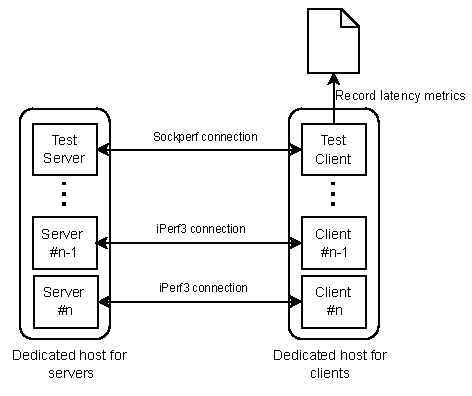
\includegraphics[width=11cm, height=9cm]{figures/latexp}
  \caption{Latency degradation experiment}
  \label{fig:latexp}
\end{figure}
\noindent
Similar to the throughput experiment, we deployed two dedicated hosts, 
one hosting all clients and one hosting all servers. Initially, only the client test node 
and its corresponding server were created. We measured the latency between them and recorded it as a baseline 
value. Subsequently, we deployed all remaining clients and incrementally increased their aggregate 
throughput in 1 Gbit/s steps (or smaller when latency degradation was observed).
This was achieved through the iPerf3 \texttt{-b} option, that allows specifying an exact throughput 
value for the client, enabling precise control over the aggregated throughput of the neighbors.
After each step, we measured the latency between the test client node and 
the test server using sockperf. The results were recorded locally on the client test node. 
Since all dedicated hosts, including the client test node and server, are located within 
the same \ac{AZ} (See Chapter \ref{chapter:infra}),
external latency variability was minimized, allowing for a better identification of latency 
degradation caused by increased throughput usage of the neighbors. \\ 